\documentclass[11pt, a4paper]{article}
\usepackage[utf8]{inputenc}
\usepackage[T1]{fontenc}
\usepackage[charter]{mathdesign} % Elegant, readable font
\usepackage{geometry}
\geometry{margin=1in}
\usepackage{enumitem}
\usepackage{amsmath}
\usepackage{booktabs}
\usepackage{hyperref}
\usepackage{graphicx} % Required for inserting images (put this in your preamble)
\usepackage{subfig}
\usepackage{comment}

\makeatletter
\renewcommand{\maketitle}{
  \begin{flushleft}
    {\huge \textbf{\@title} \par}
    \vspace{0.5cm}
    {\large \@author \par}
    \vspace{0.2cm}
    {\@date \par}
    \vspace{0.2cm}
    \hrule
  \end{flushleft}
}
\makeatother

\title{\LARGE\textbf{Molecular dynamics: 2D Lennard-Jones Simulation} \\[-0.2em]}
\author{
    Plabon Shaha and Guillem Masdemont \\ 
    \small University of Ljubljana, Spring Semester, EMAI Cohort 25--27 
}

\begin{document}

\maketitle

\begin{enumerate}
  \item[\textbf{Implementation}] We parallelize the algorithm and present several versions that are built on top of each other. We compare the speedup performance with the baseline model. We consider the following $4$ improved models:

\begin{itemize}
    \item \textbf{V1 -- CPU baseline:} All computation runs sequentially on the CPU.
    Forces are computed with an $O(n^2)$ nested loop, counting each pair twice.

    \item \textbf{V2 -- OpenMP CPU:} Same $O(n^2)$ force computation as V1 but
    parallelised across CPU cores with OpenMP. Each pair is visited once using
    Newton's third law, with per-thread scratch arrays to avoid race conditions.

    \item \textbf{V3 -- GPU 2D grid:} Force computation is offloaded to the GPU
    using a 2D thread grid where each thread handles one $(i,j)$ pair. Integration
    stays on the CPU, and GPU memory is allocated and freed every step.

    \item \textbf{V4 -- GPU 1D pairs:} Force computation uses a 1D kernel
    with one thread per unique pair and applies Newton's third law to halve the work.
    Integration still runs on the CPU with per-step memory transfers.

    \item \textbf{V5 -- Fully GPU, AoS:} All steps — forces, integration, and
    energy computation — run on the GPU. Memory is allocated once and data never
    leaves the device during the simulation loop.

    \item \textbf{V6 -- Fully GPU, SoA:} Identical to V5 but uses a
    Structure-of-Arrays memory layout, enabling contiguous memory access patterns
    across threads and reducing the number of force evaluations via $r^2$ comparisons.

    \item \textbf{V7 -- GPU neighbour list:} Introduces a Verlet neighbour list
    that limits force computation to nearby particles only, breaking the $O(n^2)$
    bottleneck. The list is rebuilt only when any particle moves more than half the
    skin thickness, amortising the rebuild cost over many steps.

    \item \textbf{V8 -- 2-GPU naive:} Particles are split evenly across two GPUs,
    each computing forces for its own half. Position data is exchanged between devices
    each step via peer-to-peer transfers where available, otherwise staged through
    the host.
\end{itemize}


\begin{figure}[h]
    \centering
    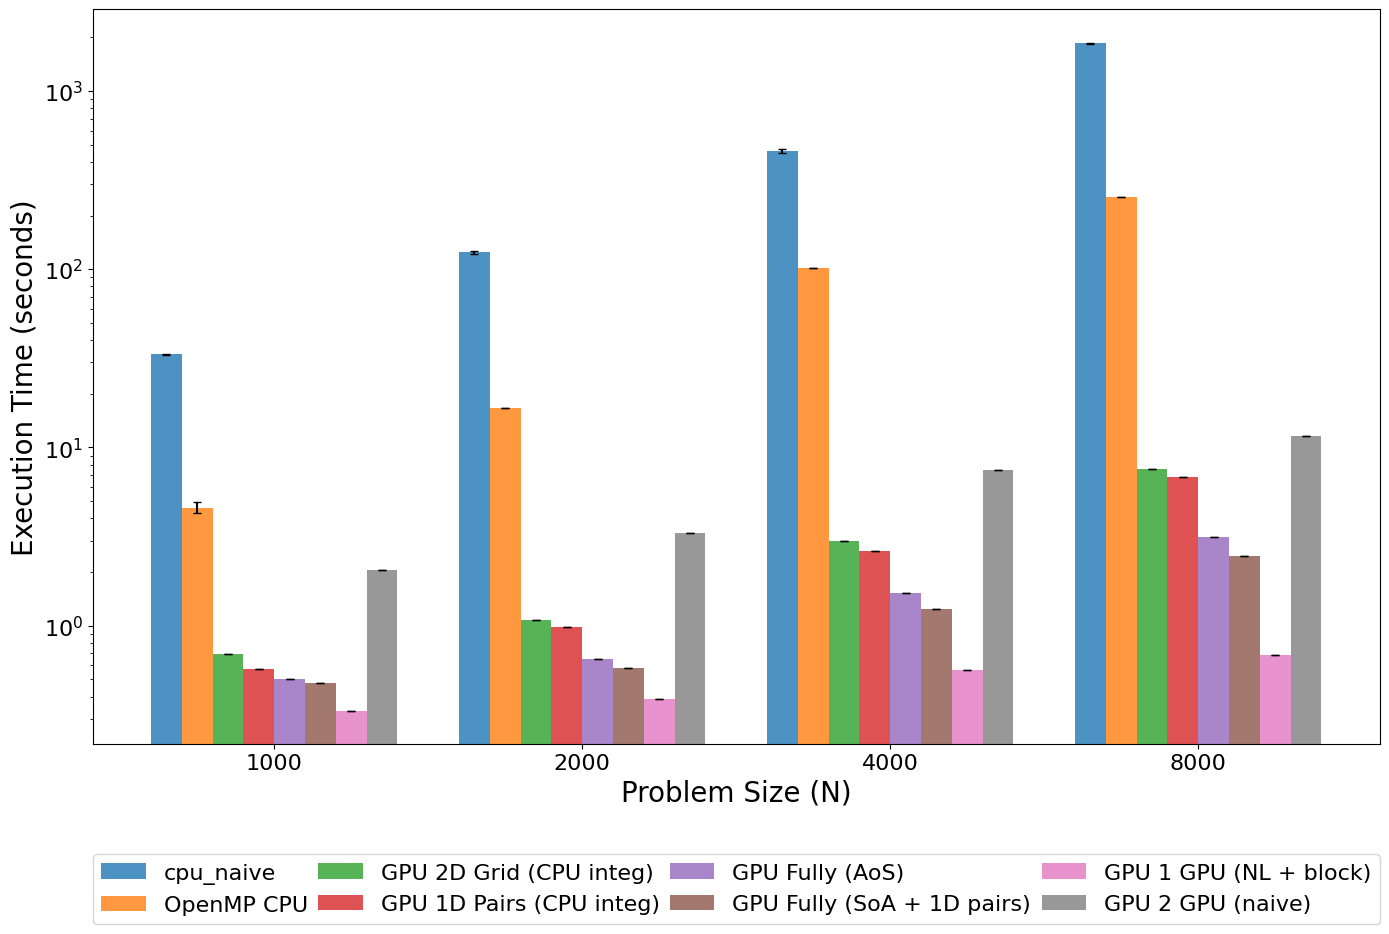
\includegraphics[width=0.9\textwidth]{performance_variance_plot.png}
    \caption{Performance comparison of the aforementioned CPU and CUDA optimization layers.}
    \label{fig:performance_plots}
\end{figure}

The results show consistent speedups as optimisations are added across all particle
counts. V3 is roughly $2\times$ faster than V2, primarily due to halving the number
of force evaluations. The largest gain comes from eliminating CPU-GPU transfers in V4,
which is $3$--$4\times$ faster than V3 at small $N$ and around $2\times$ at $N=8000$.
V5 adds a further $1.03$--$1.32\times$ improvement over V4, with the gain growing
with $N$ as coalesced memory access becomes more beneficial at larger problem sizes.
Overall, V5 achieves a $3.6$--$8.1\times$ speedup over V2 depending on particle count.
To make results meaningful, we also study the standard deviation. We observed a high standard deviation in V2, which is likely due to variable overhead from
repeated memory allocation and deallocation each step.
\end{enumerate}

\end{document}